\documentclass{article}
\usepackage{comment}
\usepackage{graphicx}
\usepackage[utf8]{inputenc}
\usepackage[english]{babel}

\begin{document}

\title{Using wavelengths outside of the Telecom spectrum}
\author{Stefan Plug\\Remy de Boer}
\date{\today}
\maketitle

\begin{comment}
\begin{tabular}{|c|c|c|}
\hline 
Version number & Date & Comment \\ 
\hline 
0.1 & 03-01-2013 & Start of of document \\ 
\hline 
\end{tabular} 
\end{comment}

\tableofcontents
\newpage

\section{Preface}
\newpage
\section{Summary}
\newpage
\section{Research question}
It is common practice today to use Wavelength Division Multiplexing, WDM, devices on network links to increase the total amount of bandwidth that a single optical network link can carry. The WDM accomplishes this by assigning each input data stream its own unique light wavelength channel, $\lambda$. 
Not every wavelength is suitable for heavy traffic usage because of the physical characteristics of these channels. Our hypothesis is that these channels could be used for lower speed applications such as monitoring and out of band management.

To test our hypothesis we will look at the possibilities of the unused wavelengths outside of the Telecom spectrum.
The main research question will be as follows:
\begin{quote}
\textit{
What applications can the unused wavelengths outside of the Telecom spectrum be used for?
}
\end{quote}

It is important to be able to have an active monitoring system in place which can send out warnings when it detects either degradation of the link over time or a sudden change in the links characteristics, for example when someone places a tap on the link. 

To help us understand how we can effectively monitor an optical link we will ask the following sub-question:
\begin{quote}
\textit{
What optical link characteristics should we monitor?
}
\end{quote}

It could happen that the main traffic interface on a switch shuts down which could potentially shut down that section of the network.
It would be good to have a separate out of band network link up on another interface which could be used to still manage that device.

During this project we will focus on link monitoring and out of band management, but other usages may arise during our research.
If this should happen we shall try to document them.

\newpage
\section{Telecom spectrum}
When we look at the wavelengths used for telecommunication we can see that the ITU-T has defined the following bands as shown in table \ref{tab:bands}
\begin{table}[h]
\centering
\label{tab:bands}
\begin{tabular}{|c|c|c|c|}
\hline 
\textbf{Band} & \textbf{Descriptor} & \textbf{Range [nm]}\\ 
\hline 
O-band & Original & 1260 to 1360 \\ 
\hline 
E-band & Extended & 1360 to 1460 \\ 
\hline 
S-band & Short wavelength & 1460 to 1530 \\ 
\hline 
C-band & Conventional & 1530 to 1565 \\ 
\hline 
L-band & Long wavelength & 1565 to 1625 \\ 
\hline 
U-band & Ultra-long wavelength & 1625 to 1675 \\ 
\hline 
\end{tabular} 
\caption{ITU-T Bands\cite[p. 134]{itu-t:manual2009}
}
\end{table}

The ITU-T further describes the U-band as:
\begin{quote}
In some cases it is desirable to perform a number of maintenance functions (preventive, after
installation, before service and post-fault) on fibre cables in the outside plant. These involve
surveillance, testing, and control activities utilizing optical time domain reflectometer (OTDR)
testing, fibre identification, loss testing, and power monitoring. A wavelength region, that is
intended to be never occupied by transmission channels, may be attractive for maintenance,
even if enhanced loss occurs. The U-band has been defined exclusively for possible
maintenance purposes.
\end{quote}

The ITU-T's intended use of the U-band corresponds with our own objectives, it is therefore obvious to us that we will further concentrate on this band.

\subsection{Choosing a wavelength}
The U-Band reaches from 1625nm to 1675nm. When choosing a wavelength we need to make sure that we have the least amount of energy loss or attenuation when transmitting light.
The amount of attenuation depends both on the fibre type and wavelength which is used. 

The main reason of our research is to look at potential uses of the unused channels at the edge of the L-band in a WDM system.
Because of this we can safely assume that the fibre optical cable used is a single mode fibre which supports C+L band WDM systems.
If the link was not used in a WDM set up, then there would be no reason to use the unconventional U-band.

The ITU-T has several standards ranging from G.652 to G.656 which specify single mode optical fibres[SOURCE], of which none have official support for the U-band.
The U-band channel we choose should for this reason be as close to the L-band as possible to keep the wavelength closer to the cable's specifications.

Figure~\ref{fig:attenuation} on page~\pageref{fig:attenuation} shows attenuation as a function of the wavelength of an unbent fibre. We can see that in the case of the U-band there is a gradual upward slope as the wavelength increases.
\begin{figure}[h]
\centerline{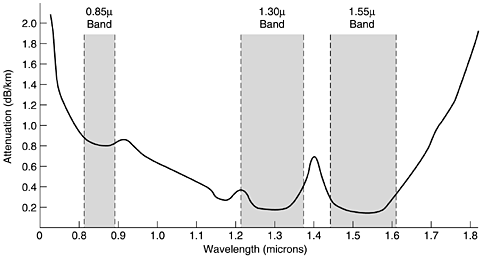
\includegraphics[scale=0.5, trim = 0mm 0mm 0mm 0mm]{images/attenuation.png}}
\caption{Attenuation of light through fibre in the infra-red region.\cite[fig 2-6]{tannenbaum:networks}}
\label{fig:attenuation}
\end{figure}

Figure~\ref{fig:attenuation-bends} on page~\pageref{fig:attenuation-bends} shows the effect of fibre bends on attenuation. Here we can see again that it is better to choose a wavelength as close to the L-band as possible.
\begin{figure}[h]
\centerline{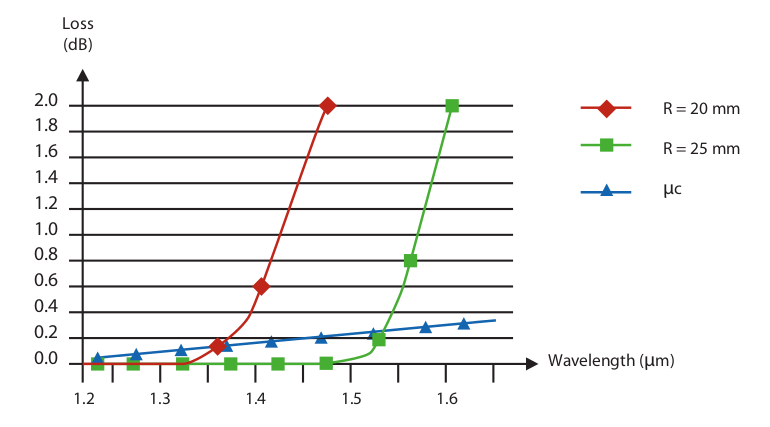
\includegraphics[scale=0.3, trim = 0mm 0mm 0mm 0mm]{images/attenuation-bends.png}}
\caption{Effect of fibre bends on attenuation.\cite[p. 27]{refguide:2011}}
\label{fig:attenuation-bends}
\end{figure}

Because the U-band begins with 1625nm we think that this would be the best wavelength to use.




\newpage
\section{Proof of Concept}
To test our hypotheses we were initially provided with two Inteno XG6746\cite{Inteno:XG6746} switches by Beetle Fiberoptics.
It is in their interest that we use this relatively cheap equipment instead of specialised, and usually more expensive fibre monitoring equipment.
The Inteno XG6746 switches have one modular SFP fibre optic port in which we can place our testing optics. 

We would like the fibre optic switches to communicate with each other so they can exchange statistics about their fibre optics and use these statistics to create MRTG\cite{MRTG:MRTG} graphs that could show interesting trends which might be an indicator of fibre degradation over time.

The Inteno XG6746 runs on the software image \texttt{XG6746\_4.02ITT24.01\_20121022}.
Because of the closed nature of the software we were not able to directly install programs or scripts which we needed to generate traffic on the fibre link directly.
Before the start of our research project we had been informed that customizable software would be made available for these switches so we could write our own testing modules.
This, however, never happened and as such we had to come up with another solution.

We tried to install several open-source operating systems on the switches, unfortunately none of them would work.
The originally installed software does allow us to read out essential information such as Rx and Tx dBm values of the optic via SNMP.

To still be able to run diagnostic tests we decided to attach a Raspberry Pi to to the switch via Ethernet which can both generate traffic and do periodic polling via SNMP.
Ideally all the functions performed by the Raspberry Pi would be integrated into the Inteno XG6746, however to simplify matters we chose to use a Raspberry Pi as it boasts a full-fledged Linux environment, Raspbian\cite{raspbian:raspbian}.

For our main tests we have used 1625nm optics.
To compare we will also run the same tests on 1470nm, 1550nm and 1610nm optics.
To validate our test-network itself we will also run similar tests on more specialised equipment using the same optics.
In theory these optics should return the same values, regardless of which equipment they are plugged into.
The optics return their values through the standardised Digital Diagnostics Monitoring, DDM\cite{SFF:DDM}, interface. This standard defines which values are measured and how the information is stored.
In practice, we have noticed that equipment manufacturers sometimes seem to change these values before displaying them.
A prime example are the Inteno switches used as the core of our tests.
The Rx and Tx values returned by these switches deviated from the actual values so much that it was impossible for us to spot any clear relation between the presented values and the values as measured by a separate optical power meter.
After some investigation our tests showed that the values presented by the Inteno switches do bear resemblance to the actual values, however they are modified in such a way as to make them completely useless.
For example: the value for Rx power actually was higher than the measured Tx value, and would even increase when the signal was purposefully attenuated.

As our initial set-up seemed unreliable for power measurements, we built another.  This time we used a 28 port ZyXEL switch to which we connected all our devices and fibres.
Using VLANs we set up connections between two Raspberry Pi's via a 25 kilometre fibre cable.
This 25 kilometre cable could then be used to test the attenuation of each signal wavelength over a reasonably long distance.

\subsection{measurable stuff}
SOMETHING ABOUT THAT WE CAN BNLY REALLY TEST ATTENUATION
\subsection{Testing equipment}

PUT ALL HARDWARE WE USED IN THIS CHAPTER INCLUDING ALL OPTICS AND OTDRs
\begin{itemize}
\item Inteno XG6746 \cite{Inteno:XG6746}
\begin{itemize}
\item Broadcom 6338
\item Marvell 88E6161
\item 8 MB Flash
\item 32 MB RAM
\end{itemize}

\item Raspberry Pi - Model B

\item Optics:
\begin{itemize}
\item SFP
\item EOptolink
\item EOLS-1603-29SD
\item 1625nm
\end{itemize}
\end{itemize}

\subsection{Primary test network}
\begin{figure}[h]
\centerline{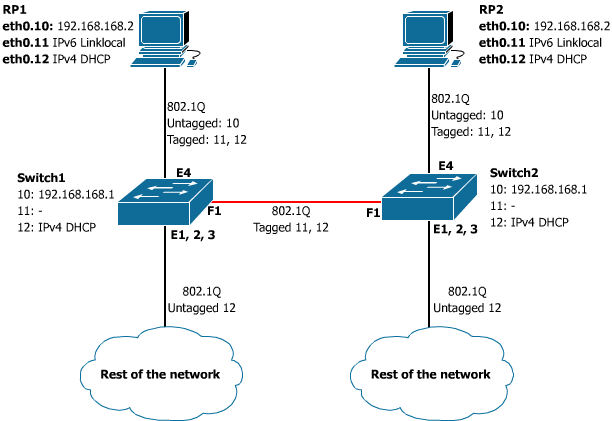
\includegraphics[scale=0.4]{images/PoC_all.png}}
\caption{Network diagram of the primary test network}
\label{fig:poc_all}
\end{figure}

Figure~\ref{fig:poc_all} on page~\pageref{fig:poc_all} shows our primary test setup which uses the Inteno XG6746 switches.
It is important to note that we use 3 separate VLANs. 

The purpose of \texttt{VLAN-10} is to create a single unit out of 1 Raspberry Pi and 1 monitored switch. This way \texttt{RP1} will only monitor \texttt{Switch1} although \texttt{Switch2} uses the same default IPv4 address as \texttt{Switch1}. In the ideal situation where the \texttt{RP\#} and \texttt{Switch\#} would be combined into 1 device this VLAN would be obsolete.

\texttt{VLAN-11} is used to exchange data between 2 \texttt{RP\#} devices. This VLAN creates a group of 2 \texttt{VLAN-10} units using the fiber optics in port \texttt{F1} on \texttt{Switch\#}. The \texttt{RP\#} devices use an IPv6 Link local address, this is done so there is no need to manually configure an IP address when 2 \texttt{VLAN-10} units are connected to each other. The 2 RPs can discover each other by sending a ping to IPv6 multicast address \texttt{FF02::1} to which all IPv6 linklocal hosts should listen and reply too\cite{ietf:rfc4291}. After the RP knows the IPv6 address of a potential neighbour it will do a simple check to see if that neighbour is indeed our polling partner and not some rouge computer. It will do this by sending a SHA256 hash of a common pre-shared password plus its own linklocal IPv6 address which should protect against a simple re-play attack.

\texttt{VLAN-12} is used to connect our devices to the rest of the network and thus might be used for out-of-band management.

\subsection{Attenuation test network}

\begin{figure}[h]
\centerline{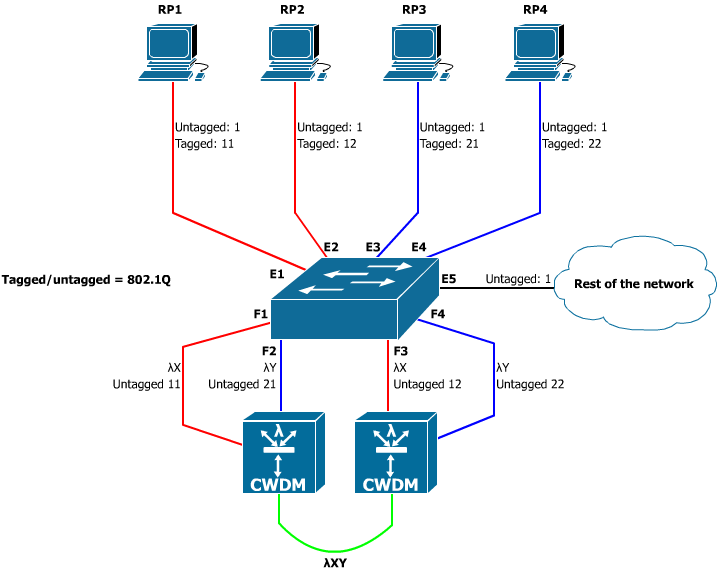
\includegraphics[scale=0.4, trim = 0mm 0mm 0mm 0mm]{images/CWDM.png}}
\caption{Network diagram of the attenuation test network}
\label{fig:CWDM}
\end{figure}

\newpage
\section{tests}
We would like to find out if we can use the 1625nm wavelength to do reliable tests of a fibre. First we will establish a base test using a well-known wavelength used for optical networking. After the base-test we will compare this to the 1625nm wavelength.

Before we will use our test-network we will test this with the reliable Bit Error Rate testers so we also have a base to compare our own set-up with.

The set of tests will consist of the following three parts:
\begin{itemize}
\item Measuring the difference between Tx and Rx values at either end of the fibre link.
	\begin{itemize}
	\item This test will be performed on the same fibre using three different sets of optics operating of different wavelengths.  We will use two common wavelengths as a base reading to compare to the results of the 1625nm wavelength.
	\end{itemize}
\item Sending a steady stream of UDP packets across the fibre at 10Mb/s.
	\begin{itemize}
	\item This will show if packets are being lost while travelling across the fibre. Our preliminary tests have shown that excessively bending a fibre will result in severe packet loss.
	\end{itemize}
\item Running traditional OTDR tests across the fibre
\end{itemize}

The first two of these tests will be done using our test set-up.
Especially for the first test it is important to bear in mind that we are getting our Tx and Rx values from the digital diagnostic information provided by the optic.
This information has an error margin which can be vendor specific, but may be at most 3dBm, as stated in the SFF-8472 Specification for
Diagnostic Monitoring Interface for Optical Transceivers\cite{SFF:DDM}






\newpage
\section{Conclusion}
\bibliographystyle{plain}
\bibliography{bibliography}

\end{document}